The given second degree equation is,
Comparing coefficients of \eqref{eq:solutions/13/94} we get,
\begin{align}
\vec{V} &= \myvec{6&\frac{1}{2}\\\frac{1}{2}&k}\\
\vec{u} &= \myvec{-\frac{11}{2}\\\frac{43}{2}}\\
f &= -35
\end{align}

The given second degree equation \eqref{eq:solutions/13/94} will represent a pair of straight line if, 
\begin{align}
\mydet{6&\frac{1}{2}&-\frac{11}{2}\\ \frac{1}{2}&k&\frac{43}{2}\\-\frac{11}{2}& \frac{43}{2}&-35}&=0\\
\intertext{Expanding the determinant,}
k+12&=0\\
\implies k&=-12\label{eq:solutions/13/95}
\end{align}
Hence, from \eqref{eq:solutions/13/95} we find that for $k=-12$, the given second degree equation \eqref{eq:solutions/13/94} represents pair of straight lines. For the appropriate value of $k$, \eqref{eq:solutions/13/94} becomes,
\begin{align}
6x^2 +xy-12y^2-11x+43y-35 = 0\label{eq:solutions/13/9main}
\end{align}

Let the pair of straight lines in vector form is given by
\begin{align}
    \vec{n_1}^T\vec{x}&=c_1\label{l1}\\
    \vec{n_2}^T\vec{x}&=c_2\label{l2}
\intertext{The pair of straight lines is given by,}
(\vec{n_1}^T\vec{x}-c_1)(\vec{n_2}^T\vec{x}-c_2) &=\vec{x}^T\vec{V}\vec{x}+2\vec{u^T}\vec{x}+f=0
\end{align}
Putting the values of $\vec{V}$ and $\vec{u}$ we get,
\begin{align}
\vec{x}^T\myvec{6&\frac{1}{2}\\\frac{1}{2}&-12}\vec{x}+2\myvec{-\frac{11}{2}&\frac{43}{2}}\vec{x}-35 &=0\label{eq:solutions/13/9line}
\end{align}
Hence, from \eqref{eq:solutions/13/9line} we get,
\begin{align}
\vec{n_1}*\vec{n_2}&=\myvec{6\\1\\-12}\label{eq:solutions/13/9conv}\\
c_2\vec{n_1}+c_1\vec{n_2}&=-2\myvec{-\frac{11}{2}\\\frac{43}{2}}\label{eq:solutions/13/9c1c2}\\
    c_1c_2&=-35
\end{align}
The slopes of the pair of straight lines are given by the roots of the polynomial,
\begin{align}
    &cm^2+2bm+a=0\label{eq:solutions/13/9quad}\\
    \implies m_i&=\frac{-b\pm{\sqrt{-\det(V)}}}{c}\\
    \vec{n_i}&=k\myvec{-m_i\\1}\label{eq:solutions/13/9slopes}
\end{align}
Substituting the values in above equations \eqref{eq:solutions/13/9quad} we get,
\begin{align}
    &-12m^2+m+6=0\\
    &\implies m_i=\frac{-\frac{1}{2}\pm{\sqrt{-(-\frac{289}{4})}}}{-12}\label{m}
\end{align}
Solving equation \eqref{m} we get ,
\begin{align}
    m_1&=-\frac{2}{3}\\
    m_2&=\frac{3}{4}\\
\intertext{Hence putting the values of $m_1$ and $m_2$ in \eqref{eq:solutions/13/9slopes} we get}
    \vec{n_1}&=k_1\myvec{\frac{2}{3}\\1}\label{eq:solutions/13/9n1}\\
    \vec{n_2}&=k_2\myvec{-\frac{3}{4} \\1}\label{eq:solutions/13/9n2}
\end{align}
Putting values of $\vec{n_1}$ and $\vec{n_2}$ in \eqref{eq:solutions/13/9conv} we get,
\begin{align}
\vec{n_1}*\vec{n_2} = \myvec{-\frac{3k_2}{4}&0\\k_2&-\frac{3k_2}{4}\\0&k_2}\myvec{\frac{2k_1}{3}\\k_1} &= \myvec{6\\1\\-12}\\
\implies\myvec{-\frac{1}{2}k_1k_2\\-\frac{1}{12}k_{1}k_{2}\\k_{1}k_{2}}&= \myvec{6\\1\\-12}\label{toeplizconv}
\end{align}
Thus, from \eqref{toeplizconv}, $k_{1}k_{2} = -12$. Possible combinations of ($k_1,k_2$) are (6,-2), (-6,2), (3,-4), (-3,4)
Lets assume $k_1=3$, $k_2=-4$, then we get, 
\begin{align}
    \vec{n_1}&=\myvec{2\\3}\label{eq:solutions/13/9n11}\\
    \vec{n_2}&=\myvec{3\\-4}\label{eq:solutions/13/9n22}
\end{align}
From equation \eqref{eq:solutions/13/9c1c2} we get 
\begin{align}
    \myvec{\vec{n_1} & \vec{n_2}}\myvec{c_2\\c_1}&=-2\vec{u}\\
    \myvec{2 & 3\\3 & -4}\myvec{c_2\\c_1}&=-2\myvec{-\frac{11}{2}\\\frac{43}{2}}\
\intertext{Hence we get the following equations,}
    2c_2+3c_1&=11\label{eq:solutions/13/9sol1}\\
    3c_2-4c_1&=-43\label{eq:solutions/13/9sol2}
\end{align}
The augmented matrix of \eqref{eq:solutions/13/9sol1} ,\eqref{eq:solutions/13/9sol2} is,
\begin{align}
\myvec{2&3&11\\3&-4&-43}&\underleftrightarrow{R_1=\frac{1}{2}R_1}\myvec{1&\frac{3}{2}&\frac{11}{2}\\3&-4&-43}\\
&\underleftrightarrow{R_2=R_2-3R_1}\myvec{1&\frac{3}{2}&\frac{11}{2}\\0&-\frac{17}{2}&-\frac{119}{2}}\\
&\underleftrightarrow{R_2=-\frac{2}{17}}\myvec{1&\frac{3}{2}&\frac{11}{2}\\0&1&7}\\
&\underleftrightarrow{R_1=R_1-\frac{3}{2}R_2}\myvec{1&0&-5\\0&1&7}\\
\end{align}
Hence we get,
\begin{align}
    c_1&=-5\\
    c_2&=7
\end{align}
Hence \eqref{l1}, \eqref{l2} can be modified as follows,
\begin{align}
    \myvec{2 & 3}\vec{x}&=-5\label{eq:solutions/13/9line1}\\
    \myvec{3 & -4}\vec{x}&=7\label{eq:solutions/13/9line2}
\end{align}
The figure below corresponds to the pair of straight lines represented by \eqref{eq:solutions/13/9line1} and \eqref{eq:solutions/13/9line2}.
\begin{figure}[h!]
\centering
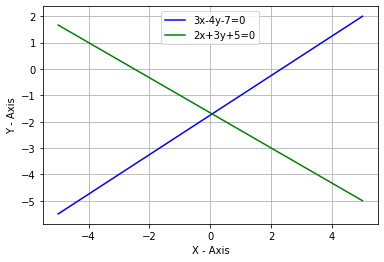
\includegraphics[width = \columnwidth]{./solutions/13/9/Lines.png}
\caption{Pair of Straight Lines}
\label{fig:solutions/13/9my_label}
\end{figure}
